\documentclass[12pt, a4paper]{report}
\usepackage[top=1cm, left=1cm, right=1cm]{geometry}

\usepackage[utf8]{inputenc}
\usepackage[russian]{babel}

\usepackage{array}
\newcolumntype{M}[1]{>{\centering\arraybackslash}m{#1}}

\usepackage{hyperref}
\hypersetup{
	colorlinks,
	citecolor=black,
	filecolor=black,
	linkcolor=black,
	urlcolor=black
}

\usepackage{sectsty}
\allsectionsfont{\centering}

\usepackage{indentfirst}
\setlength\parindent{24pt}

\usepackage{algorithm}
\usepackage[noend]{algpseudocode}

\usepackage{listings}
\usepackage{xcolor}
\definecolor{codegreen}{rgb}{0,0.6,0}
\definecolor{codegray}{rgb}{0.5,0.5,0.5}
\definecolor{codepurple}{rgb}{0.58,0,0.82}
\definecolor{backcolour}{rgb}{0.95,0.95,0.92}
\lstdefinestyle{mystyle}{
    backgroundcolor=\color{backcolour},   
    commentstyle=\color{codegreen},
    keywordstyle=\color{magenta},
    numberstyle=\normalsize\color{codegray},
    stringstyle=\color{codepurple},
    basicstyle=\ttfamily\footnotesize,
    breakatwhitespace=false,         
    breaklines=true,                 
    captionpos=b,                    
    keepspaces=true,                 
    numbers=left,                    
    numbersep=5pt,                  
    showspaces=false,                
    showstringspaces=false,
    showtabs=false,                  
    tabsize=2
}

\usepackage{graphicx}
\graphicspath{{plots/pictures/}}

\begin{document}
	\begin{titlepage}
		\begin{center}
			\large \textbf{Министерство науки и высшего образования Российской Федерации} \\
			\large \textbf{Федеральное государственное бюджетное образовательное учреждение высшего образования} \\
			\large \textbf{«Российский химико-технологический университет имени Д.И. Менделеева»} \\

			\vspace*{4cm}
			\LARGE \textbf{ОТЧЕТ ПО ЛАБОРАТОРНОЙ РАБОТЕ №2}

			\vspace*{4cm}
			\begin{flushright}
				\Large
				\begin{tabular}{>{\raggedleft\arraybackslash}p{9cm} p{10cm}}
					Выполнил студент группы КС-36: & Золотухин А.А. \\
					Ссылка на репозиторий: & https://github.com/ \\
					& MUCTR-IKT-CPP/ \\
					& ZolotukhinAA\_36\_ALG \\
					Принял: & Крашенников Роман Сергеевич \\
					Дата сдачи: & 03.03.2025 \\
				\end{tabular}
			\end{flushright}

			\vspace*{6cm}
			\Large \textbf{Москва \\ 2025}
		\end{center}
	\end{titlepage}

	\tableofcontents
	\thispagestyle{empty}
	\newpage

	\pagenumbering{arabic}

	\section*{Описание задачи}
	\addcontentsline{toc}{section}{Описание задачи}
	\large
	В лабораторной работе предлагается изучить альтернативные первой лабораторной работы сортировки, которые обладают меньшей асимптотической сложностью и сравнить их с результатами предыдущей лабораторной работы. \par
	Используя предыдущий код посерийного выполнения алгоритма сортировки и измерения времени требуется реализовать метод пирамидальной сортировки. \par
	Задание:
	\begin{itemize}
		\item Реализовать проведения тестирования алгоритма сериями расчётов для измерения параметров времени. \par
		За один расчёт выполняются следующие операции:
		\begin{enumerate}
			\item Генерируется массив случайных значений;
			\item Запоминается время начала расчёта алгоритма сортировки;
			\item Выполняется алгоритм сортировки
			\item Вычисляется время, затраченное на сортировку: текущее время - время начала;
			\item Сохраняется время для одной попытки. \par
			После этого расчёт повторяется до окончания серии.
			\begin{itemize}
				\item Алгоритм вычисляется 8 сериями по 20 раз за серию;
				\item Алгоритм в каждой серии вычисляется для массива размером M (1000,2000, 4000, 8000, 16000, 32000, 64000, 128000);
				\item Массив заполняется значениями чисел с плавающей точкой в интервале от -1 до 1;
				\item Для серии запоминаются все времена, которые были замерены.
			\end{itemize}
		\end{enumerate}
		\item По полученным данным времени построить графики зависимости времени от числа элементов в массиве:
		\begin{enumerate}
			\item Совмещенный график наихудшего времени выполнения сортировки и сложности алгоритма, указанной в нотации O большое; \par
			Для построения графика вычисляется O большое для каждого размера массива. При этом при вычислении функции O(c * g(N)) подбирается такая константа c, чтобы при значении >1000 график O(N) был выше графика наихудшего случая, но второй график на его фоне не превращался в прямую линию.
			\item Совмещенный график среднего, наихудшего и наилучшего времени исполнения;
			\item Совмещённый график средней, наилучшей и наихудшей глубины рекурсии;
			\item Совмещённый график среднего по серии количество вызовов функции построения кучи и количества вызовов внутренней функции;
			\item График среднего процентного соотношения вызовов внутренней функции к общему вызову функции.
		\end{enumerate}
		\item По результатам расчётов оформляется отчёт по предоставленной форме, в отчете:
		\begin{enumerate}
			\item Приводится описание алгоритма;
			\item Приводится описание выполнения задачи (описание кода и специфических элементов реализации);
			\item Приводятся выводы (Графики и их анализ). Требуется ответить на вопрос о поведении алгоритма, изученного в процессе выполнения лабораторной работы и зафиксировать его особенности.
		\end{enumerate}
	\end{itemize}

	\section*{Описание метода/модели}
	\addcontentsline{toc}{section}{Описание метода/модели}
	\large
	\textit{Пирамидальная сортировка (или, Сортировка кучей)} - это метод сортировки на основе сравнения, основанный на двоичной куче данных. При сортировке кучей мы используем двоичную кучу, чтобы быстро находить и перемещать максимальный элемент за \textit{O(logN)} вместо \textit{O(N)} и, следовательно, достигать временной сложности \textit{O(NlogN)}.
	Ход алгоритма:
	\begin{enumerate}
		\item Переставляем элементы массива так, чтобы они образовывали максимальную кучу;
		\item Повторяем следующие шаги до тех пор, пока куча не будет содержать только один элемент:
		\begin{enumerate}
			\item Меняем местами корневой элемент кучи с последним элементом кучи;
			\item Удаляем последний элемент кучи;
			\item Складываем в кучу остальные элементы кучи.
		\end{enumerate}
		\item Получаем отсортированный массив.
	\end{enumerate}
	Анализ сложности пирамидальной сортировки:
	\begin{itemize}
		\item \textbf{Лучший вариант: O(\( N \))}, если массив уже отсортирован;
		\item \textbf{Средний вариант: O(\( N(logN) \))}, если массив упорядочен случайным образом;
		\item \textbf{Наихудший вариант: O(\( N(logN) \))}, если массив находится в обратном порядке, \par
		где N - количество элементов в массиве.
	\end{itemize}
	\textit{Преимущества}:
	\begin{itemize}
		\item Эффективная временная сложность;
		\item Использование памяти может быть минимальным;
		\item Простота.
	\end{itemize}
	\textit{Недостатки}:
	\begin{itemize}
		\item Дорогостоящая, так как константы выше по сравнению с сортировкой слиянием;
		\item Неэффективен из-за высоких констант во временной сложности.
	\end{itemize}

	\section*{Выполнение задачи}
	\addcontentsline{toc}{section}{Выполнение задачи}
	Алгоритм пирамидальной сортировки реализован на языке \textit{C++}. Построение графиков проводить с помощью программы \textit{GNUplot}.

	\textit{"main"} функция работает с циклом, в ходе которого производится расчёт минимального, максимального и среднего времени на сортировку массива размером \textit{M}. Каждая серия просчитывается по 20 раз. В итоге получаются данные, выведенные в определенные файлы, с помощью которых впоследствии строятся графики.
	\lstset{style=mystyle}
	\begin{lstlisting}[language=C++]
		int main() {
		    std::ofstream worst_and_complexity(Constants::folder + "worst_and_complexity.dat");
		    std::ofstream average_best_worst(Constants::folder + "average_best_worst.dat");
		    std::ofstream recursion_depth(Constants::folder + "recursion_depth.dat");
		    std::ofstream heap_calls(Constants::folder + "heap_calls.dat");
		    std::ofstream inner_heap_ratio(Constants::folder + "inner_heap_ratio.dat");

		    if (!worst_and_complexity.is_open() ||
			!average_best_worst.is_open() ||
			!recursion_depth.is_open() ||
			!heap_calls.is_open() ||
			!inner_heap_ratio.is_open()) {
			std::cerr << "Error of opening file!" << std::endl;
			return 1;
		    }

		    for (int episode = 0; episode < Constants::M; episode++) {
			int size = Constants::sizes[episode];
			double* array = new double[size];

			long double the_worst_time = 0.0;
			long double the_best_time = std::numeric_limits<long double>::max();
			long double total_time = 0.0;

			long long total_heap_calls_all = 0;
			long long total_inner_heap_calls_all = 0;
			long long max_recursion_depth_all = 0;

			long double total_recursion_depth = 0.0;
			long double best_recursion_depth = std::numeric_limits<long double>::max();
			long double worst_recursion_depth = 0.0;

			for (int attempt = 0; attempt < Constants::amount_of_attempts; attempt++) {
			    long long total_heap_calls = 0;
			    long long total_inner_heap_calls = 0;
			    long long current_depth = 0;
			    long long max_recursion_depth = 0;

			    generationArray(array, size);

			    std::chrono::high_resolution_clock::time_point start = std::chrono::high_resolution_clock::now();

			    heapSort(array, size, total_heap_calls, total_inner_heap_calls, max_recursion_depth);

			    std::chrono::high_resolution_clock::time_point end = std::chrono::high_resolution_clock::now();
			    std::chrono::duration<long double, std::milli> milli_diff = end - start;

			    long double time_taken = milli_diff.count();
			    if (time_taken > the_worst_time)
				the_worst_time = time_taken;
			    if (time_taken < the_best_time)
				the_best_time = time_taken;

			    total_time += time_taken;
			    total_heap_calls_all += total_heap_calls;
			    total_inner_heap_calls_all += total_inner_heap_calls;

			    if (max_recursion_depth > max_recursion_depth_all)
				max_recursion_depth_all = max_recursion_depth;

			    total_recursion_depth += max_recursion_depth;
			    if (max_recursion_depth < best_recursion_depth)
				best_recursion_depth = max_recursion_depth;
			    if (max_recursion_depth > worst_recursion_depth)
				worst_recursion_depth = max_recursion_depth;

			    std::cout << "Time: " << time_taken << " ms." << std::endl;
			}

			long double average_time = total_time / Constants::amount_of_attempts;
			long double complexity = Constants::c * static_cast<long double>(size) * std::log(size);
			std::cout << complexity << std::endl;

			long double average_heap_calls = static_cast<long double>(total_heap_calls_all) / Constants::amount_of_attempts;
			long double average_inner_heap_calls = static_cast<long double>(total_inner_heap_calls_all) / Constants::amount_of_attempts;
			long double inner_heap_ratio_value = (average_inner_heap_calls / average_heap_calls) * 100.0;

			long double average_recursion_depth = total_recursion_depth / Constants::amount_of_attempts;

			worst_and_complexity << size << " " << the_worst_time << " " << complexity << std::endl;
			average_best_worst << size << " " << average_time << " " << the_best_time << " " << the_worst_time << std::endl;
			recursion_depth << size << " " << average_recursion_depth << " " << best_recursion_depth << " " << worst_recursion_depth << std::endl;
			heap_calls << size << " " << average_heap_calls << " " << average_inner_heap_calls << std::endl;
			inner_heap_ratio << size << " " << inner_heap_ratio_value << std::endl;

			delete[] array;
		    }

		    worst_and_complexity.close();
		    average_best_worst.close();
		    recursion_depth.close();
		    heap_calls.close();
		    inner_heap_ratio.close();

		    return 0;
		}
	\end{lstlisting}
	\par
	\textit{"generationArray"} функция принимает два аргумента: array - массив, size - размер массива. Формирует массив размера size, который заполняется случайными числами с плавающей точкой от -1 до 1.
	\lstset{style=mystyle}
	\begin{lstlisting}[language=C++]
		void generationArray(double array[], int size) {
			std::random_device rd;
			std::mt19937 engine(rd());
			std::uniform_real_distribution<double> gen(-1.0, 1.0);

			for (int i = 0; i < size; i++)
				array[i] = gen(engine);
		}		
	\end{lstlisting}
	\par
	\textit{"heapSort"} функция принимает пять аргументов: array - массив, size - размер массива, total\_heap\_calls - общее число вызовов кучи, total\_inner\_heap\_calls - общее число внутренних вызовов кучи, max\_recursion\_depth - максимальная глубина рекурсии. Сортирует массив пирамидальным методом и просчитывает общее число вызовов кучи, общее число внутренних вызовов кучи и максимальную глубину рекурсии.
	\lstset{style=mystyle}
	\begin{lstlisting}[language=C++]
		void heapSort(double array[], int size, long long& total_heap_calls, long long& total_inner_heap_calls, long long& max_recursion_depth) {
		    for (int i = (size / 2 - 1); i >= 0; i--) {
			long long current_depth = 0;
			makeHeap(array, size, i, total_heap_calls, total_inner_heap_calls, current_depth, max_recursion_depth);
		    }

		    for (int i = (size - 1); i >= 0; i--) {
			std::swap(array[0], array[i]);
			long long current_depth = 0;
			makeHeap(array, i, 0, total_heap_calls, total_inner_heap_calls, current_depth, max_recursion_depth);
		    }
		}
	\end{lstlisting}
	\par
	\textit{"makeHeap"} функция принимает 6 аргументов: array - массив, size - размер массива, i - текущий индекс, total\_heap\_calls - общее число вызовов кучи, total\_inner\_heap\_calls - общее число внутренних вызовов кучи, max\_recursion\_depth - максимальная глубина рекурсии. Создаёт "максимальную" кучу для неупорядоченного массива и просчитывает общее число вызовов кучи, общее число внутренних вызовов кучи и максимальную глубину рекурсии.
	\lstset{style=mystyle}
	\begin{lstlisting}[language=C++]
		void makeHeap(double array[], int size, int i, long long& total_heap_calls, long long& total_inner_heap_calls, long long& current_depth, long long& max_recursion_depth) {
		    total_heap_calls++;
		    current_depth++;

		    if (current_depth > max_recursion_depth)
			max_recursion_depth = current_depth;

		    int largest = i;
		    int l = 2 * i + 1;
		    int r = 2 * i + 2;

		    if (l < size && array[l] > array[largest])
			largest = l;

		    if (r < size && array[r] > array[largest])
			largest = r;

		    if (largest != i) {
			std::swap(array[i], array[largest]);
			makeHeap(array, size, largest, total_heap_calls, total_inner_heap_calls, current_depth, max_recursion_depth);
			total_inner_heap_calls++;
		    }
		}
	\end{lstlisting}

	\newpage
	\vfill

	\begin{figure}
		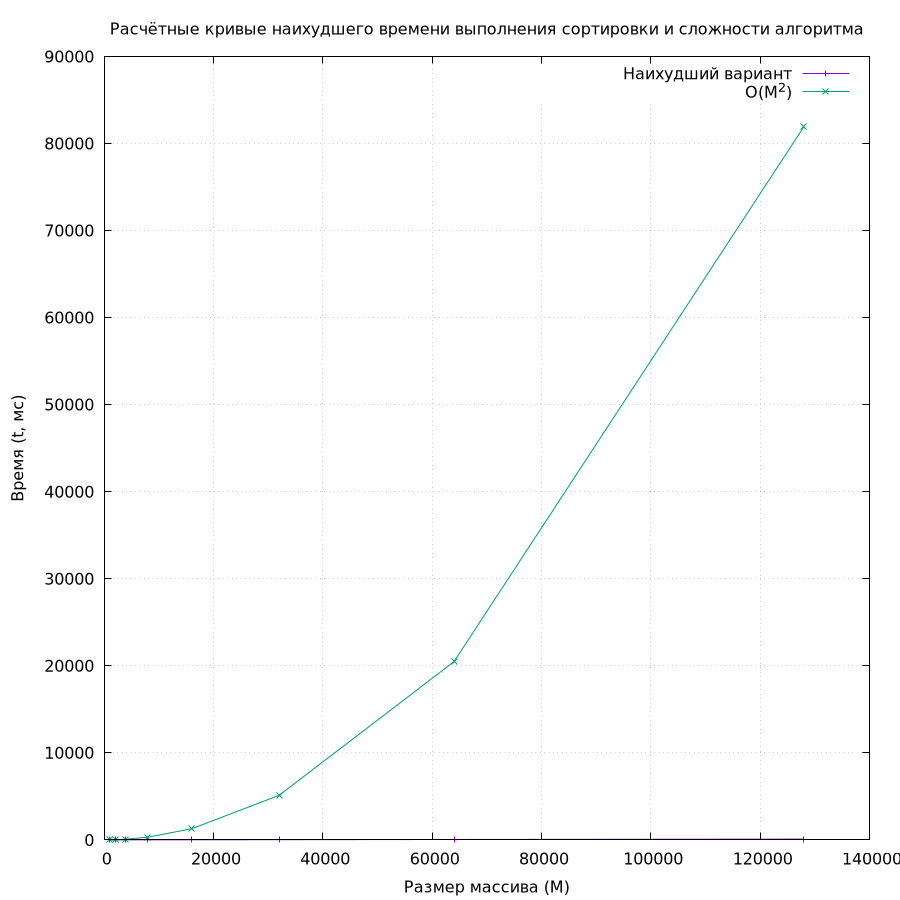
\includegraphics[width=300pt]{worst_and_complexity.png}
	\end{figure}
	\begin{figure}
		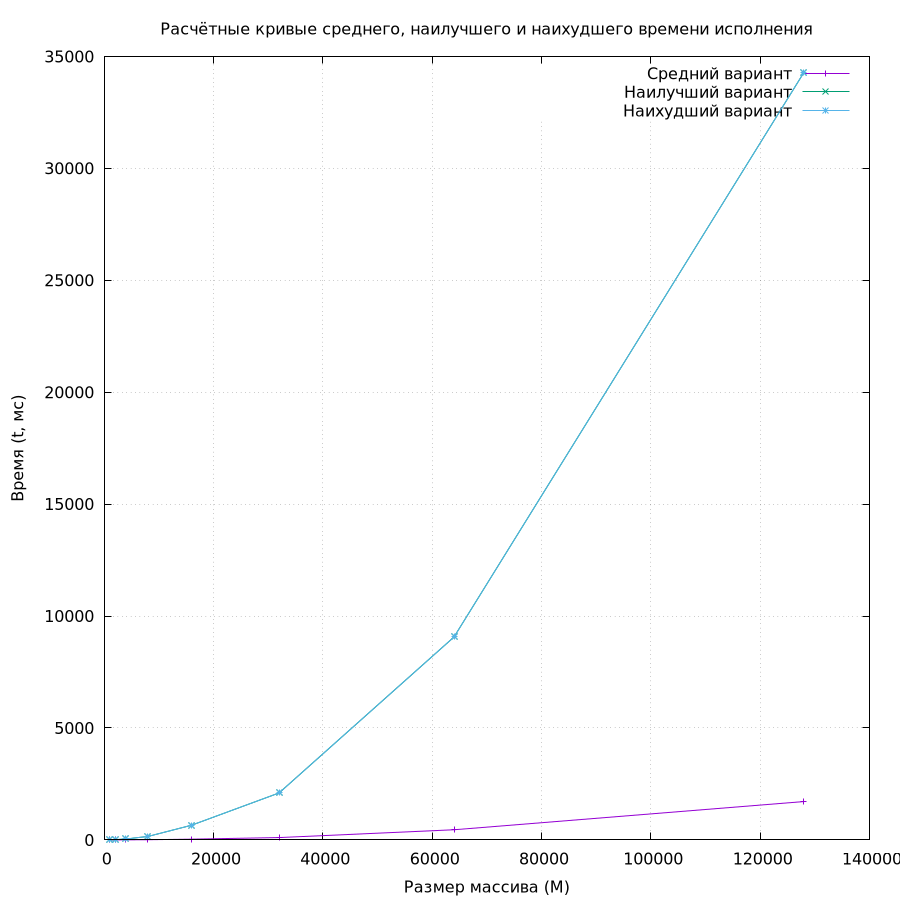
\includegraphics[width=300pt]{average_best_worst.png}
	\end{figure}
	\begin{figure}
		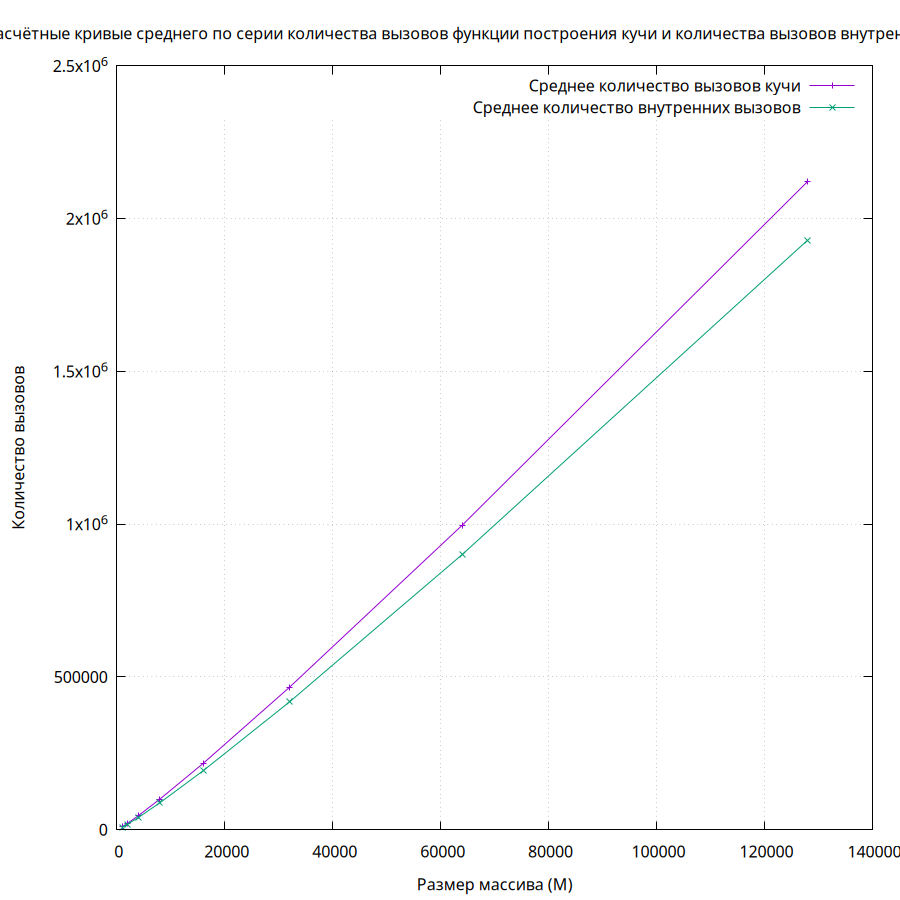
\includegraphics[width=300pt]{heap_calls.png}
	\end{figure}
	\begin{figure}
		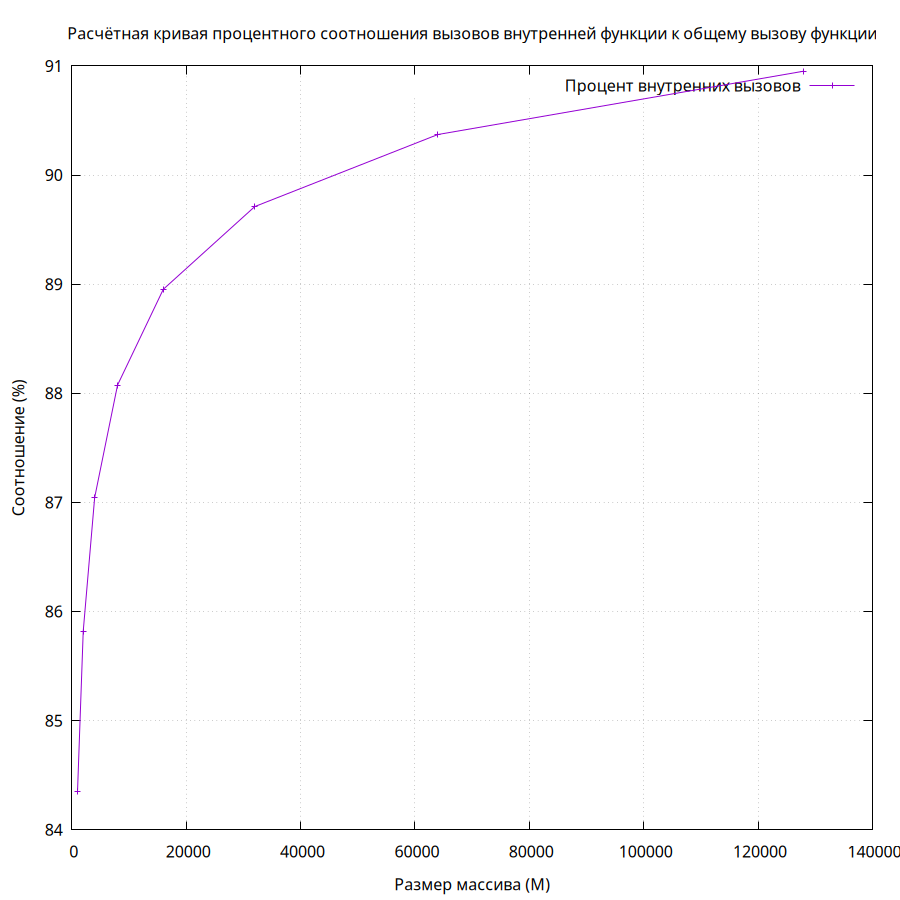
\includegraphics[width=300pt]{inner_heap_ratio.png}
	\end{figure}

	\vfill
	\clearpage

	\section*{Выводы}
	\addcontentsline{toc}{section}{Выводы}

\end{document}
